\documentclass[graybox]{svmult}
%%
%% NOTE this file is a slightly modified version of the 'author.tex' file
%% provided in the 'templates' directory in the springer latex package.
%% I have made changes (a) to conform to the style selected for the PT-AI
%% Proceedings volume, as specified in http://www.pt-ai.org/2013/submission
%% If you find any errors or infelicities, please inform Aaron Sloman
%% by email:  a.sloman@cs.bham.ac.uk
%%
%%
%% If you don't need to use boxes of text with a gray background, illustrated
%% in this example (search for "svgraybox"), then start your latex file
%%with the following:
%% \documentclass[]{svmult}
%%
%% NOTE: Some of the text that was previously in the referenc.tex file
%% has been moved into this file, since that file was not consistent
%% with use of bibtex to generate the bibliography.
%%
\usepackage{mathptmx}       % selects Times Roman as basic font
\usepackage{helvet}         % selects Helvetica as sans-serif font
\usepackage{courier}        % selects Courier as typewriter font
\usepackage{type1cm}        % activate if the above 3 fonts are
%%%%%%%%%%%%%%%%%%%% author.tex %%%%%%%%%%%%%%%%%%%%%%%%%%%%%%%%%%%
%
% sample root file for your "contribution" to a contributed volume
%
% Use this file as a template for your own input.
%
% %%%%%%%%%%%%%%% Springer %%%%%%%%%%%%%%%%%%%%%%%%%%%%%%%%%%


% RECOMMENDED %%%%%%%%%%%%%%%%%%%%%%%%%%%%%%%%%%%%%%%%%%%%%%%%%%%

%% for use in connection with the recommended bibliography style

%% use the file spbasic.bst, and the natbib latex package
\bibliographystyle{spbasic}
\usepackage{natbib}
%%
%% Better bibliography formatting is provided by apacite, if available.
%% But that can be left to Springer
%\bibliographystyle{apacite}
%\usepackage{apacite}


% choose options for [] as required from the list
% in the Reference Guide
                            % not available on your system

%%% not needed for PT-AI
%%\usepackage{makeidx}         % allows index generation

\usepackage{graphicx}        % standard LaTeX graphics tool
                             % when including figure files
\usepackage{multicol}        % used for the two-column index
%% Probably not needed?

\usepackage[bottom]{footmisc}% places footnotes at page bottom

% see the list of further useful packages
% in the Reference Guide

%% Not needed for PT-AI contributions.
%%\makeindex           % used for the subject index
                       % with the style svind.ist with

% Use the "url.sty" package to prevent formatting problems in urls, e.g. in
% institution address or used in your e-mail or web address or Bibliography
%% avoids problems with special characters
\usepackage{url}

%%%%%%%%%%%%%%%%%%%%%%%%%%%%%%%%%%%%%%%%%%%%%%%%%%%%%%%%%%%%%%%%%%%%%%%%%%%%%%%%%%%%%%%%%

\begin{document}

%% INSERT YOUR PAPER TITLE HERE
\title*{Sample PT-AI Author Contribution}
% Use \titlerunning{Short Title} for an abbreviated version of for an abbreviated version of
% your contribution title if the original one is too long
\titlerunning{Author Contribution}
%%
\author{Name of First Author and Name of Second Author}
% Use \authorrunning{Name} for an abbreviated version of for an abbreviated version of
% author name if the original one is too long
\authorrunning{First and Second Authors}
%
%% Edit as appropriate for one or more authors
\institute{Name of First Author \at Name1, Address of Institute1, \email{nam1e@email.address}
\and Name of Second Author \at Name2, Address of Institute2 \email{name2@email.address}}
%
%
\maketitle

%% remove this comment

\vspace*{-2cm}

\noindent
{{\bf NOTE:} \em This PDF file was generated from pt-ai-author.tex (a modified
version of the author.tex file in the Springer ``templates'' directory), using also
author.bib, svmult.cls (Springer multi-author style file), the natbib latex style and
Springer spbasic.bst (Springer bibliography and citation style file).}
\\[2mm]

\abstract*{Each
chapter should be preceded by an abstract (10--15 lines long) that summarizes the
content. The abstract will appear \textit{online} at \url{www.SpringerLink.com} and
be available with unrestricted access. This allows unregistered users to read the
abstract as a teaser for the complete chapter. As a general rule the abstracts will
not appear in the printed version of your book unless it is the style of your
particular book or that of the series to which your book belongs. Please use the
'starred' version of the new Springer \texttt{abstract} command for typesetting the
text of the online abstracts (cf. source file of this chapter template
\texttt{abstract}) and include them with the source files of your manuscript. Use the
plain \texttt{abstract} command if the abstract is also to appear in the printed
version of the book.}

\abstract{Each
chapter should be preceded by an abstract (10--15 lines long) that summarizes the
content. The abstract will appear \textit{online} at \url{www.SpringerLink.com} and
be available with unrestricted access. This allows unregistered users to read the
abstract as a teaser for the complete chapter. As a general rule the abstracts will
not appear in the printed version of your book unless it is the style of your
particular book or that of the series to which your book belongs.\newline\indent
Please use the 'starred' version of the new Springer \texttt{abstract} command for
typesetting the text of the online abstracts (cf. source file of this chapter
template \texttt{abstract}) and include them with the source files of your
manuscript. Use the plain \texttt{abstract} command if the abstract is also to appear
in the printed version of the book. Use both for PT-AI chapters. This is the
un-starred abstract.}

\section{Section Heading}
\label{sec:1}

Use the template \emph{pt-ai-author.tex} together with the Springer document class
SVMult (for edited books) to style the various elements of your chapter content in
the Springer layout.

Much of this text is nonsense copied from the Springer author sample file. Some of it
explains how the formatting is done, however.

Instead of simply listing headings of different levels we recommend to let every
heading be followed by at least a short passage of text. Please also use the \LaTeX\
mechanisms for all your cross-references and citations. And please note that the
first line of text that follows a heading is not indented, whereas the first lines of
all subsequent paragraphs are.

\section{Section Heading}
\label{sec:2}
% Always give a unique label
% and use \ref{<label>} for cross-references
% and \cite{<label>} for bibliographic references
% use \sectionmark{}
% to alter or adjust the section heading in the running head
Instead of simply listing headings of different levels we recommend to
let every heading be followed by at least a short passage of text.
Further, please also use the \LaTeX\ and BibTeX mechanisms for all your
cross-references, citations and bibliography listing.

Please note that the first line of text that follows a heading is not indented, whereas the first lines of all subsequent paragraphs are.

Use the standard \verb|equation| environment to typeset your equations, e.g.
%
\begin{equation}
a \times b = c\;,
\end{equation}
%
however, for multiline equations we recommend to use the \verb|eqnarray| environment\footnote{In physics texts please activate the class option \texttt{vecphys} to depict your vectors in \textbf{\itshape boldface-italic} type - as is customary for a wide range of physical subjects}.
\begin{eqnarray}
a \times b = c \nonumber\\
\vec{a} \cdot \vec{b}=\vec{c}
\label{eq:01}
\end{eqnarray}

\subsection{Subsection Heading}
\label{subsec:2}
Instead of simply listing headings of different levels we recommend to
let every heading be followed by at least a short passage of text.

Please also use the \LaTeX\ mechanisms for all your
cross-references\index{cross-references} and citations\index{citations}
as has already been described in Sect.~\ref{sec:2}.

\begin{quotation}
Please do not use quotation marks when quoting texts! Simply use the \verb|quotation|
environment -- it will automatically render Springer's preferred layout, as in this
example paragraph.
\end{quotation}


\subsubsection{Subsubsection Heading}
Instead of simply listing headings of different levels we recommend to
let every heading be followed by at least a short passage of text.
Further on please use the \LaTeX\ mechanisms for all your
cross-references and citations as has already been described in
Sect.~\ref{subsec:2}, see also Fig.~\ref{fig:1}\footnote{If you copy
text passages, figures, or tables from other works, you must obtain
\textit{permission} from the copyright holder (usually the original
publisher). Please enclose the signed permission with the manucript. The
sources\index{permission to print} must be acknowledged either in the
captions, as footnotes or in a separate section of the book.}

Please note that the first line of text that follows a heading is not indented,
whereas the first lines of all subsequent paragraphs are.


\paragraph{Paragraph Heading} %
Instead of simply listing headings of different levels we recommend to
let every heading be followed by at least a short passage of text.
Further on please use the \LaTeX\ mechanisms for all your
cross-references and citations as has already been described in
Sect.~\ref{sec:2}.

Please note that the first line of text that follows a heading is not indented, whereas the first lines of all subsequent paragraphs are.

For typesetting numbered lists we recommend to use the \verb|enumerate| environment -- it will automatically render Springer's preferred layout.

\begin{enumerate}
\item{Livelihood and survival mobility are oftentimes outcomes of uneven socioeconomic development.}
\begin{enumerate}
\item{Livelihood and survival mobility are oftentimes outcomes of uneven socioeconomic development.}
\item{Livelihood and survival mobility are oftentimes outcomes of uneven socioeconomic development.}
\end{enumerate}
\item{Livelihood and survival mobility are oftentimes outcomes of uneven socioeconomic development.}
\end{enumerate}


% For figures use
%
\begin{figure}[h]
%% Try to insert the figure 'here' (!h), If it does not fit, it may be placed at
%% the top of the next page.
% Use the relevant command for your figure-insertion program
% to insert the figure file.
% For example, with the graphicx style use this, to get the figure centred.
\centerline{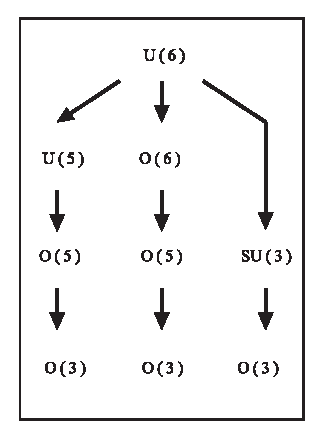
\includegraphics[scale=0.8]{figure}}
%
% If no graphics program available, insert a blank space i.e. use
%\picplace{5cm}{2cm} % Give the correct figure height and width in cm
%
\caption{This is how a normal figure caption will appear, below the figure. Another
example is given below in Fig.~\ref{fig:2}, using the \texttt{sidecaption}
command. }
\label{fig:1}       % Give a unique label
\end{figure}

\subparagraph{Subparagraph Heading}
In order to avoid simply listing headings of different levels we recommend letting
every heading be followed by at least a short passage of text.


\subparagraph{Cross-references}
Use the \LaTeX\ mechanisms for all your cross-references and citations as has already
been described
in Sect.~\ref{sec:2}, see also Fig.~\ref{fig:1} and Fig.~\ref{fig:2}.
In contrast, Sect.~\ref{sec:subsec} illustrates a subsection reference.


\subparagraph{Unnumbered lists}
For unnumbered list we recommend to use the \verb|itemize| environment -- it will automatically render Springer's preferred layout.

\begin{itemize}
\item{Livelihood and survival mobility are oftentimes outcomes of uneven socioeconomic development, cf. Table~\ref{tab:1}.}
\begin{itemize}
\item{Livelihood and survival mobility are oftentimes outcomes of uneven socioeconomic development.}
\item{Livelihood and survival mobility are oftentimes outcomes of uneven socioeconomic development.}
\end{itemize}
\item{Livelihood and survival mobility are oftentimes outcomes of uneven socioeconomic development.}
\end{itemize}




\begin{figure}[t]
\sidecaption[t]
% Use the relevant command for your figure-insertion program
% to insert the figure file.
% For example, with the option graphics use
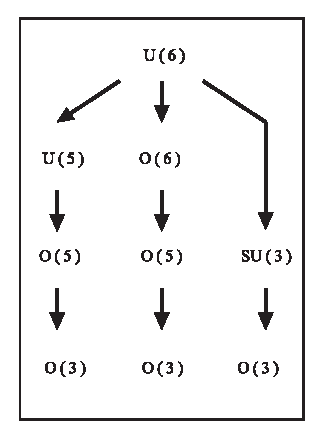
\includegraphics[scale=.65]{figure}
%
% If no graphics program available, insert a blank space i.e. use
%\picplace{5cm}{2cm} % Give the correct figure height and width in cm
%
%\caption{Please write your figure caption here}
\caption{If the width of the figure is less than 7.8 cm use the \texttt{sidecapion} command
to set the caption flush on the left side of the page. If the figure is positioned at
the top of the page, align the sidecaption with the top of the figure -- to achieve
this you simply need to use the optional argument \texttt{[t]} with the
\texttt{sidecaption} command}
\label{fig:2}       % Give a unique label
\end{figure}

\runinhead{Run-in Heading Boldface Version}
Use the \LaTeX\ mechanisms for all your cross-references and citations as has already been described in Sect.~\ref{sec:2}.

\subruninhead{Run-in Heading Italic Version} Use the \LaTeX\ mechanisms for all your cross-refer\-ences and citations as has already been described in Sect.~\ref{sec:2}\index{paragraph}.
% Use the \index{} command to code your index words
%
% For tables use
%
\begin{table}
\caption{Please write your table caption here}
\label{tab:1}       % Give a unique label
%
% Follow this input for your own table layout
%
\begin{tabular}{p{2cm}p{2.4cm}p{2cm}p{4.9cm}}
\hline\noalign{\smallskip}
Classes & Subclass & Length & Action Mechanism  \\
\noalign{\smallskip}\svhline\noalign{\smallskip}
Translation & mRNA$^a$  & 22 (19--25) & Translation repression, mRNA cleavage\\
Translation & mRNA cleavage & 21 & mRNA cleavage\\
Translation & mRNA  & 21--22 & mRNA cleavage\\
Translation & mRNA  & 24--26 & Histone and DNA Modification\\
\noalign{\smallskip}\hline\noalign{\smallskip}
\end{tabular}
$^a$ Table foot note (with superscript)
\end{table}
%
\section{Section Heading}
\label{sec:3}
% Always give a unique label
% and use \ref{<label>} for cross-references
% and \cite{<label>} for bibliographic references
% use \sectionmark{}
% to alter or adjust the section heading in the running head
Instead of simply listing headings of different levels we recommend to
let every heading be followed by at least a short passage of text.
Further on please use the \LaTeX\ mechanisms for all your
cross-references and citations as has already been described in
Sect.~\ref{sec:2}.
In contrast, Sect.~\ref{sec:subsec} illustrates a subsection reference.

Please note that the first line of text that follows a heading is not indented, whereas the first lines of all subsequent paragraphs are.

If you want to list definitions or the like we recommend to use the Springer-enhanced \verb|description| environment -- it will automatically render Springer's preferred layout.

\begin{description}[Type 1]
\item[Type 1]{That addresses central themes pertainng to migration, health, and disease. In Sect.~\ref{sec:1}, Wilson discusses the role of human migration in infectious disease distributions and patterns.}
\item[Type 2]{That addresses central themes pertainng to migration, health, and disease. In Sect.~\ref{subsec:2}, Wilson discusses the role of human migration in infectious disease distributions and patterns.}
\end{description}

\subsection{Subsection Heading} %
\label{sec:subsec}
In order to avoid simply listing headings of different levels we recommend to let every heading be followed by at least a short passage of text. Use the \LaTeX\ mechanisms for all your cross-references and citations citations as has already been described in Sect.~\ref{sec:2}.

Please note that the first line of text that follows a heading is not indented, whereas the first lines of all subsequent paragraphs are.

\begin{svgraybox}
If you want to emphasize complete paragraphs of texts we recommend to use the newly defined Springer class option \verb|graybox| and the newly defined environment \verb|svgraybox|. This will produce a 15 percent screened box
`behind' your text.

If you want to emphasize complete paragraphs of texts we recommend to use the newly defined Springer class option and environment \verb|svgraybox|. This will produce a 15 percent screened box
`behind' your text.
\end{svgraybox}


\subsubsection{Subsubsection Heading}
Instead of simply listing headings of different levels we recommend to
let every heading be followed by at least a short passage of text.
Further on please use the \LaTeX\ mechanisms for all your
cross-references and citations as has already been described in
Sect.~\ref{sec:2}.

Please note that the first line of text that follows a heading is not indented,
whereas the first lines of all subsequent paragraphs are.

\begin{theorem}
Theorem text goes here.
\end{theorem}
%
% or
%
\begin{definition}
Definition text goes here.
\end{definition}

\begin{proof}
%\smartqed
Proof text
\\goes here.
\\
\qed
\end{proof}

\paragraph{Paragraph Heading} %
Instead of simply listing headings of different levels we recommend to
let every heading be followed by at least a short passage of text.
Further on please use the \LaTeX\ mechanisms for all your
cross-references and citations as has already been described in
Sect.~\ref{sec:2}.

Note that the first line of text that follows a heading is not indented, whereas the first lines of all subsequent paragraphs are.
%
% For built-in environments use
%
\begin{theorem}
Theorem text goes here.
\end{theorem}
%
\begin{definition}
Definition text goes here.
\end{definition}
%
\begin{proof}
\smartqed
Proof text goes here.
\qed
\end{proof}
%
\begin{acknowledgement}
If you want to include acknowledgments of assistance and the like at the end of an individual chapter please use the \verb|acknowledgement| environment -- it will automatically render Springer's preferred layout.
\end{acknowledgement}
%
\section*{Appendix}
\addcontentsline{toc}{section}{Appendix}
%
%
When placed at the end of a chapter or contribution (as opposed to at the end of the book),
the numbering of tables, figures, and equations in the appendix section continues on from
that in the main text. Hence please \textit{do not} use the \verb|appendix| command when
writing an appendix at the end of your chapter or contribution.
If there is only one the appendix is designated ``Appendix'', or ``Appendix 1'', or
``Appendix 2'', etc. if there is more than one.

\begin{equation}
a \times b = c
\end{equation}

\begin{equation}
X \times Y = Z
\end{equation}

\section{Reference Formats}

References may be \textit{cited} in the text by author/year.\footnote{Make
sure that all references from the list are cited in the text.
Those not cited should be moved to a separate \textit{Further Reading}
section or chapter.}
The reference list should be \textit{sorted} in alphabetical order.
If there are several works by the same author, the following order should be used:
\begin{enumerate}
\item all works by the author alone, ordered chronologically by year of publication
\item all works by the author with a coauthor, ordered alphabetically by coauthor
\item all works by the author with several coauthors, ordered chronologically by year of publication.
\end{enumerate}
The \textit{styling} of references\footnote{Always use the standard abbreviation of a journal's name according to the ISSN \textit{List of Title Word Abbreviations}, see \url{http://www.issn.org/en/node/344}}
depends on the subject of your book:
\begin{itemize}
\item The \textit{two} recommended styles for references in books on \textit{mathematical, physical, statistical and computer sciences} are
not depicted here.
\item Examples of the basic Springer style, \texttt{spbasic},
used in the PT-AI proceedings
are \cite{calfee-1991}, \cite{dod-1999}, \cite{harris-et-al}, and
\cite{oneil-et-al}
\end{itemize}

%% Bibliography
%% If you have a list references pre-built in a file referenc.tex you may need this.
%% See the example referenc.tex file in the templates directory ../templates/
%\input{referenc}
%% Alternatively use a file in bibtex input format, like the authour.bib file
%% provided, and referenced below.

%

\small

%%Author's bibtex file author.bib is used here
\bibliography{author}

\runinhead{Note:} This bibliography was generated from the \texttt{author.bib}
bibliography file, using {\em bibtex}.
\end{document}
